\begin{figure}[H]
    \centering
    \begin{subfigure}{0.1\textwidth} 
        \raisebox{2.2\height}{\includegraphics[width=\linewidth]{data/heat_hex/0.png}} \caption{} 
    \end{subfigure}
    \hspace{0.5em}
    \begin{subfigure}{0.28\textwidth}
        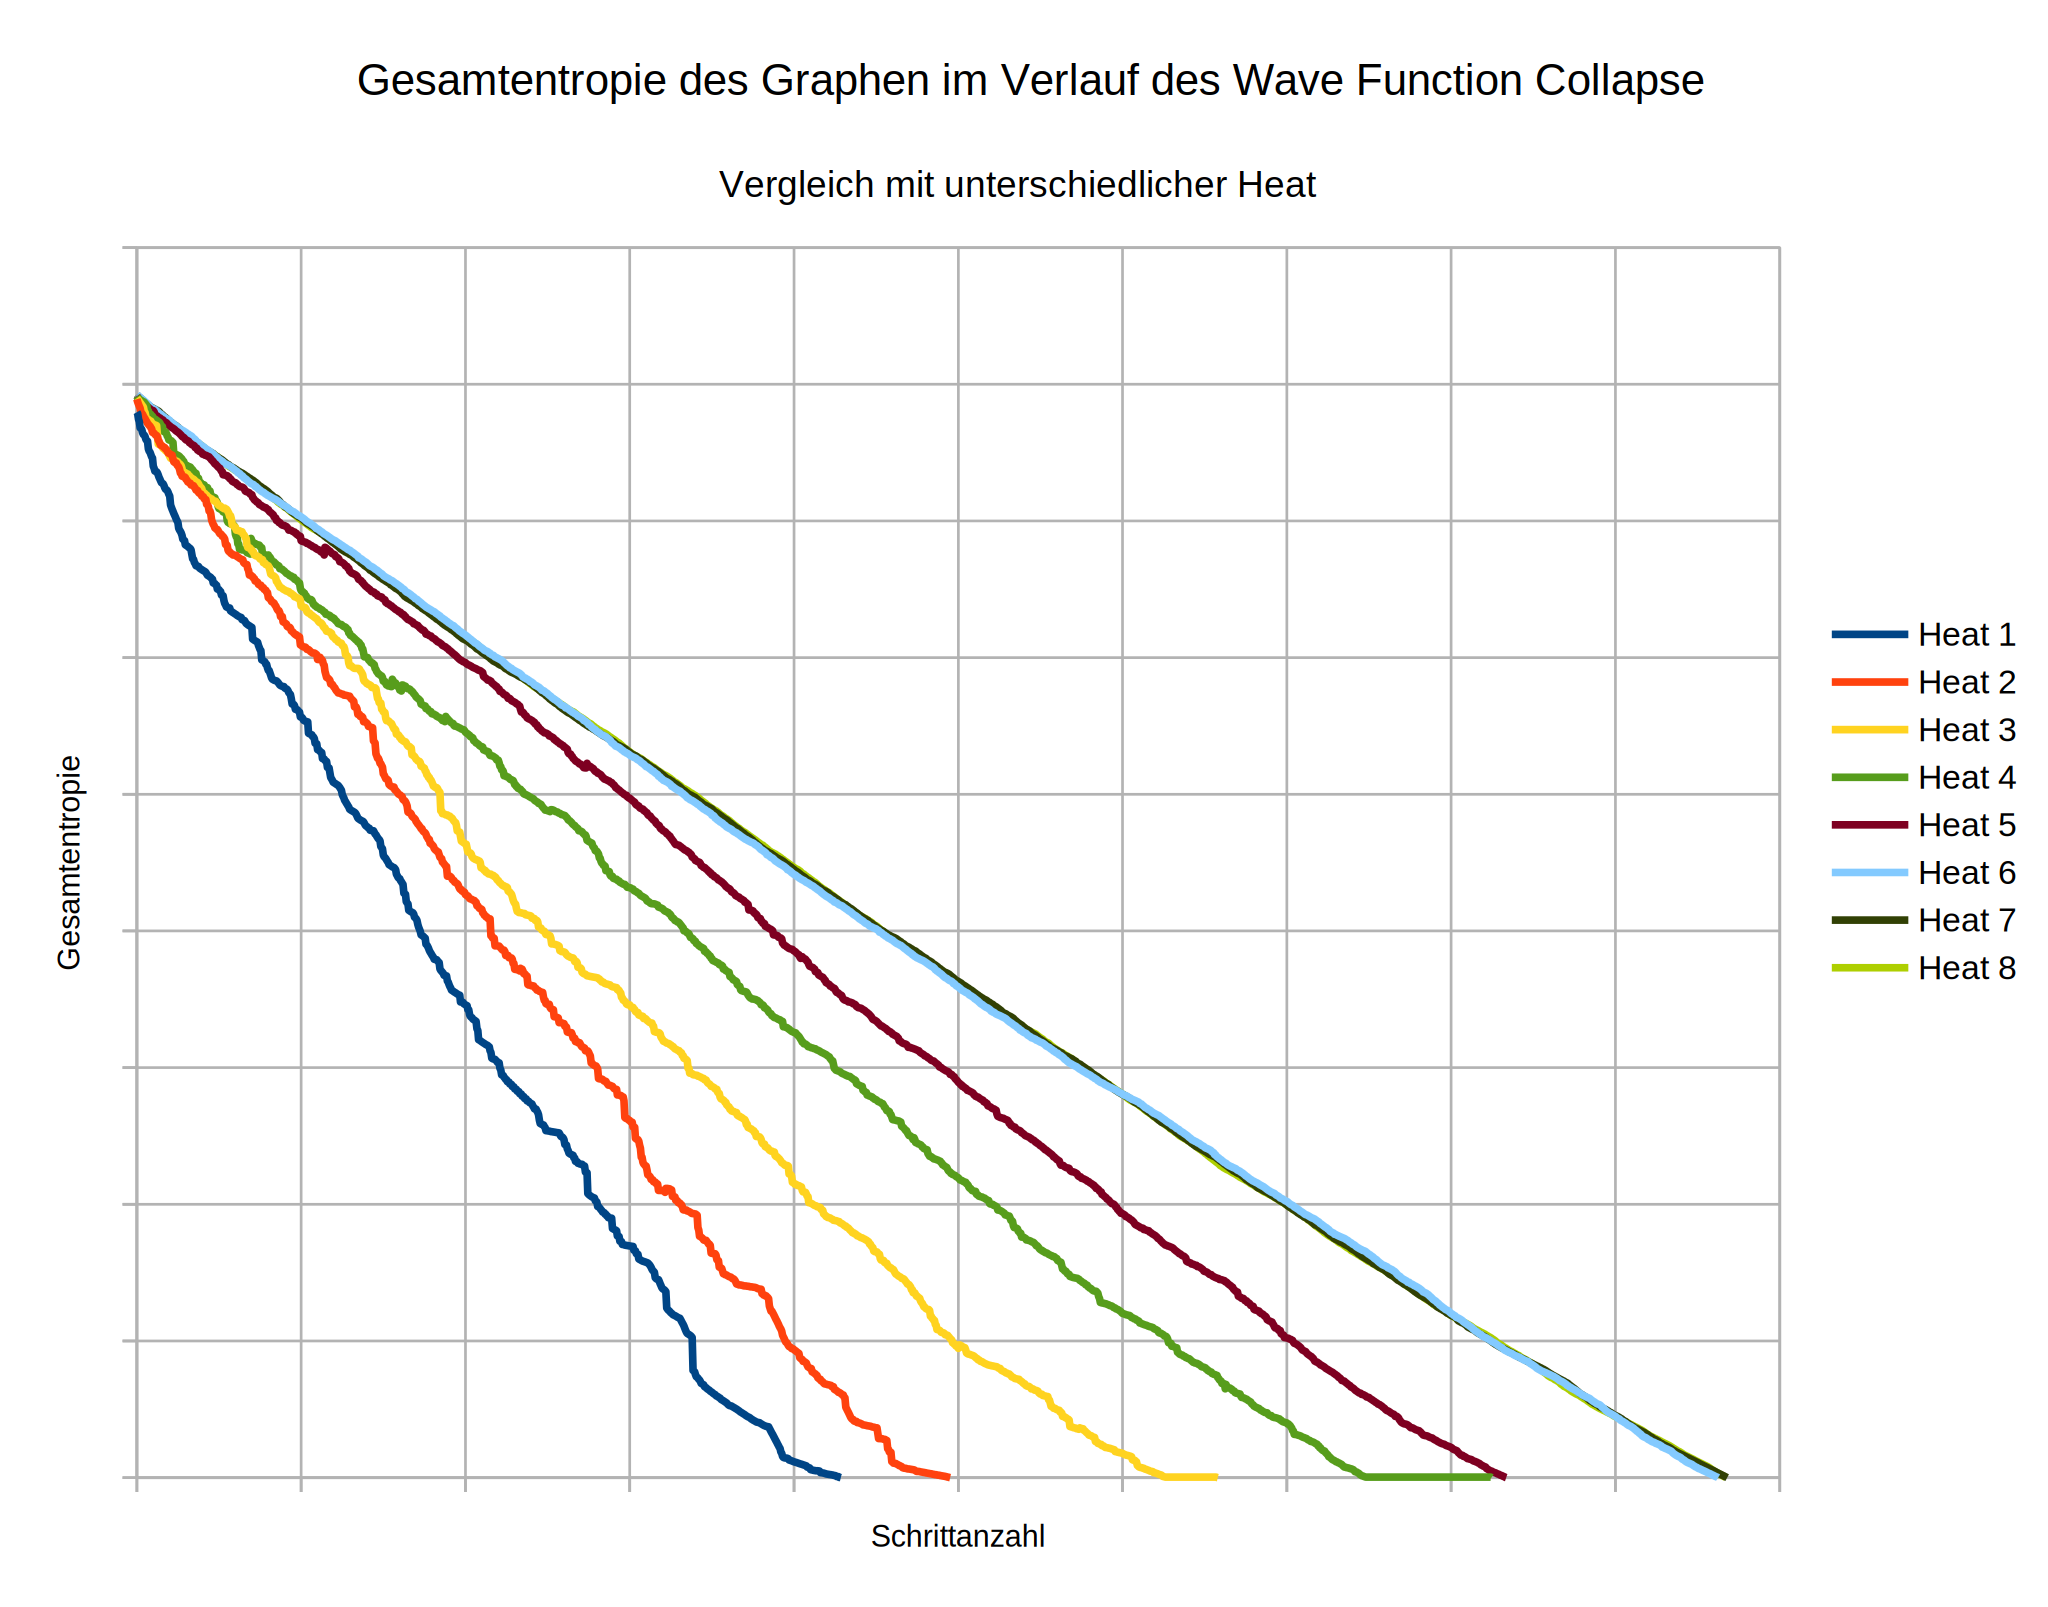
\includegraphics[width=\linewidth]{data/heat_hex/1.png} \caption{}
    \end{subfigure}\hfill
    \begin{subfigure}{0.28\textwidth}
        \includegraphics[width=\linewidth]{data/heat_hex/2.png} \caption{}
    \end{subfigure}
    \begin{subfigure}{0.28\textwidth}
        \includegraphics[width=\linewidth]{data/heat_hex/3.png} \caption{}
    \end{subfigure}\hfill
    
    \caption{
        Einfluss von Heat auf die Qualität der Ausgabe. (a) Beispielbild. (b) Quadratgitter mit Heat=1. (c) Sechseckgitter mit Heat=1. (d) Secheckgitter mit Heat=2.
    }
    \label{fig:heat_hex}
\end{figure}